\documentclass[aspectratio=169]{beamer}

\usetheme{default}
\setbeamertemplate{navigation symbols}{}
\usepackage{tikz}
\usetikzlibrary{arrows.meta,positioning,fit,calc}

\title{N-gram Speculative Decoding Implementation}
\author{Jia Guo}
\date{}

\begin{document}

\begin{frame}
  \titlepage
\end{frame}

\begin{frame}{N-gram matching and extending}
  \centering
  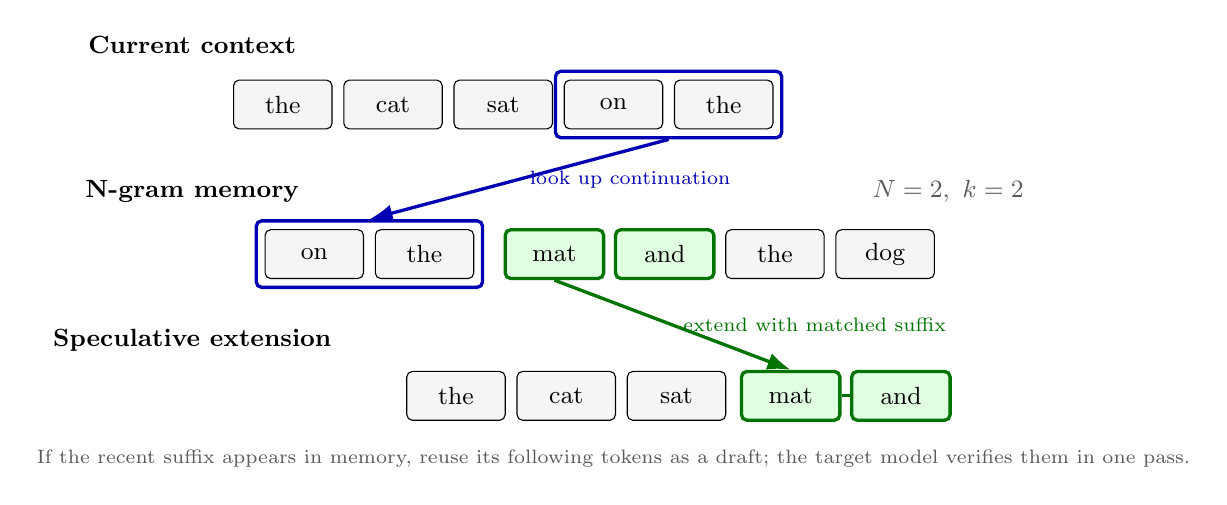
\begin{tikzpicture}[
      >=Latex,
      token/.style={draw, rounded corners=2pt, minimum width=1.25cm,
        minimum height=0.62cm, font=\small, fill=gray!8},
      match/.style={token, draw=blue!70!black, very thick, fill=blue!10},
      next/.style={token, draw=green!45!black, very thick, fill=green!12},
      label/.style={font=\small\bfseries, align=left},
      arrow/.style={->, very thick, draw=black!65}
    ]

    % Current context
    \node[label] at (-5.35,2.1) {Current context};
    \node[token] (c1) at (-4.2,1.35) {the};
    \node[token] (c2) at (-2.8,1.35) {cat};
    \node[token] (c3) at (-1.4,1.35) {sat};
    \node[token] (c4) at (0.0,1.35) {on};
    \node[token] (c5) at (1.4,1.35) {the};
    \node[match, fill=none, fit=(c4)(c5), inner sep=3pt,
      label={[blue!70!black]above:{matched 2-gram}}] (ctxmatch) {};

    % N-gram memory
    \node[label] at (-5.35,0.25) {N-gram memory};
    \node[font=\small, text=black!65] at (4.25,0.25) {$N = 2,\ k = 2$};
    \node[token] (m1) at (-3.8,-0.55) {on};
    \node[token] (m2) at (-2.4,-0.55) {the};
    \node[next] (m3) at (-0.75,-0.55) {mat};
    \node[next] (m4) at (0.65,-0.55) {and};
    \node[token] (m5) at (2.05,-0.55) {the};
    \node[token] (m6) at (3.45,-0.55) {dog};
    \node[match, fill=none, fit=(m1)(m2), inner sep=3pt] (memmatch) {};

    \draw[arrow, blue!70!black] (ctxmatch.south) -- node[right, font=\scriptsize,
      align=left] {look up continuation} (memmatch.north);

    % Extension
    \node[label] at (-5.35,-1.65) {Speculative extension};
    \node[token] at (-2.0,-2.35) {the};
    \node[token] at (-0.6,-2.35) {cat};
    \node[token] at (0.8,-2.35) {sat};
    \node[next] (e1) at (2.25,-2.35) {mat};
    \node[next] (e2) at (3.65,-2.35) {and};
    \draw[arrow, green!45!black] (m3.south) -- node[right, font=\scriptsize]
      {extend with matched suffix} (e1.north);
    \draw[green!45!black, very thick, dashed] (e1.east) -- (e2.west);

    \node[font=\scriptsize, text=black!65, align=center] at (0,-3.15)
      {If the recent suffix appears in memory, reuse its following tokens as a draft; the target model verifies them in one pass.};
  \end{tikzpicture}
\end{frame}

\begin{frame}{Speculative decoding: greedy verification and KV cleanup}
  \centering
  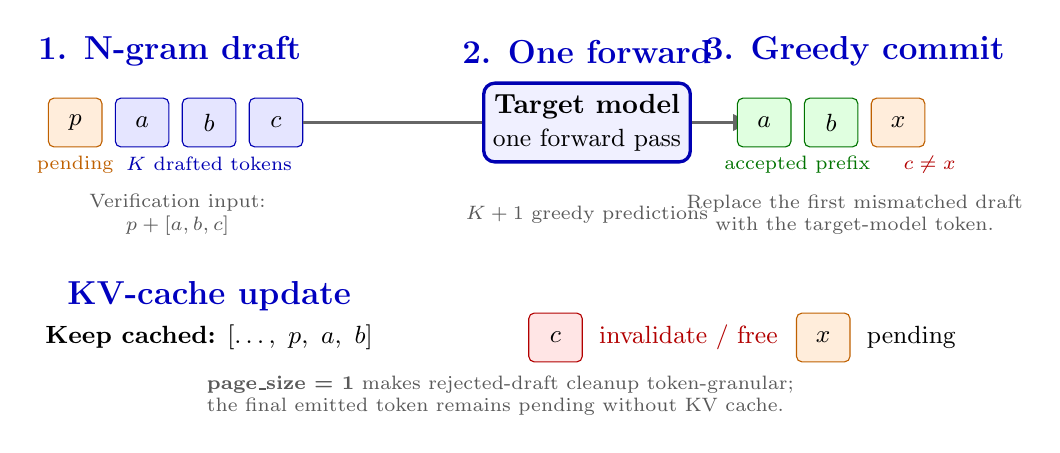
\begin{tikzpicture}[
      >=Latex,
      flow/.style={->, very thick, draw=black!60},
      token/.style={draw, rounded corners=2pt, minimum width=0.68cm,
        minimum height=0.62cm, font=\small, fill=gray!8},
      draft/.style={token, draw=blue!70!black, fill=blue!10},
      accept/.style={token, draw=green!45!black, fill=green!12},
      reject/.style={token, draw=red!70!black, fill=red!10},
      pending/.style={token, draw=orange!75!black, fill=orange!14},
      heading/.style={font=\large\bfseries, text=blue!75!black},
      caption/.style={font=\scriptsize, text=black!65, align=center}
    ]
    % Draft
    \node[heading] at (-4.35,2.05) {1. N-gram draft};
    \node[pending] (p) at (-5.55,1.15) {$p$};
    \node[draft] (da) at (-4.7,1.15) {$a$};
    \node[draft] (db) at (-3.85,1.15) {$b$};
    \node[draft] (dc) at (-3.0,1.15) {$c$};
    \node[font=\scriptsize, text=orange!75!black] at (-5.55,0.62) {pending};
    \node[font=\scriptsize, text=blue!70!black] at (-3.85,0.62) {$K$ drafted tokens};
    \node[caption] at (-4.25,-0.02) {Verification input:\\$p + [a,b,c]$};

    % Verify
    \draw[flow] (dc.east) -- (0.0,1.15);
    \node[heading] at (0.95,2.05) {2. One forward};
    \node[draw=blue!70!black, very thick, rounded corners=4pt,
      fill=blue!6, minimum width=2.25cm, minimum height=1.0cm, align=center]
      (model) at (0.95,1.15) {\textbf{Target model}\\\small one forward pass};
    \node[caption] at (0.95,-0.02) {$K+1$ greedy predictions};

    % Greedy compare
    \draw[flow] (model.east) -- (3.1,1.15);
    \node[heading] at (4.35,2.05) {3. Greedy commit};
    \node[accept] (pa) at (3.2,1.15) {$a$};
    \node[accept] (pb) at (4.05,1.15) {$b$};
    \node[pending] (px) at (4.9,1.15) {$x$};
    \node[font=\scriptsize, text=green!45!black] at (3.62,0.62)
      {accepted prefix};
    \node[font=\scriptsize, text=red!70!black] at (5.3,0.62)
      {$c \ne x$};
    \node[caption] at (4.35,-0.02)
      {Replace the first mismatched draft\\with the target-model token.};

    % Cache state
    \node[heading] at (-3.85,-1.05) {KV-cache update};
    \node[font=\small, align=left] at (-3.85,-1.58)
      {\textbf{Keep cached:} $[\ldots,\ p,\ a,\ b]$};
    \node[reject] (freec) at (0.55,-1.58) {$c$};
    \node[font=\small, text=red!70!black, anchor=west] at (0.98,-1.58)
      {invalidate / free};
    \node[pending] at (3.95,-1.58) {$x$};
    \node[font=\small, anchor=west] at (4.38,-1.58) {pending};
    \node[caption, align=left] at (-0.15,-2.32)
      {\textbf{page\_size = 1} makes rejected-draft cleanup token-granular;\\
       the final emitted token remains pending without KV cache.};
  \end{tikzpicture}
\end{frame}

\begin{frame}{Design decisions}
  \vspace{0.45cm}
  \begin{itemize}
    \setlength{\itemsep}{0.75cm}
    \item \textbf{Request-local lookup:} search only the current request's context.
    \item \textbf{N-gram fallback:} if $N=3$ has no match, retry $N=2$, then $N=1$.
    \item \textbf{Page size = 1:} Mini-SGLang's default; enables token-level
      KV-cache cleanup after rejected drafts.
    \item \textbf{Fold decode into verification:} scheduling has prefill and
      verification steps only---no separate decode step.
  \end{itemize}
\end{frame}

\begin{frame}{Verification and forward-prep optimizations}
  \small
  \textcolor{black!65}{Four profiler snapshots across the optimization sequence.}

  \vspace{0.18cm}
  \begin{columns}[T,onlytextwidth]
    \begin{column}{0.49\textwidth}
      \textbf{Baseline --- pure decoding}

      \vspace{0.06cm}
      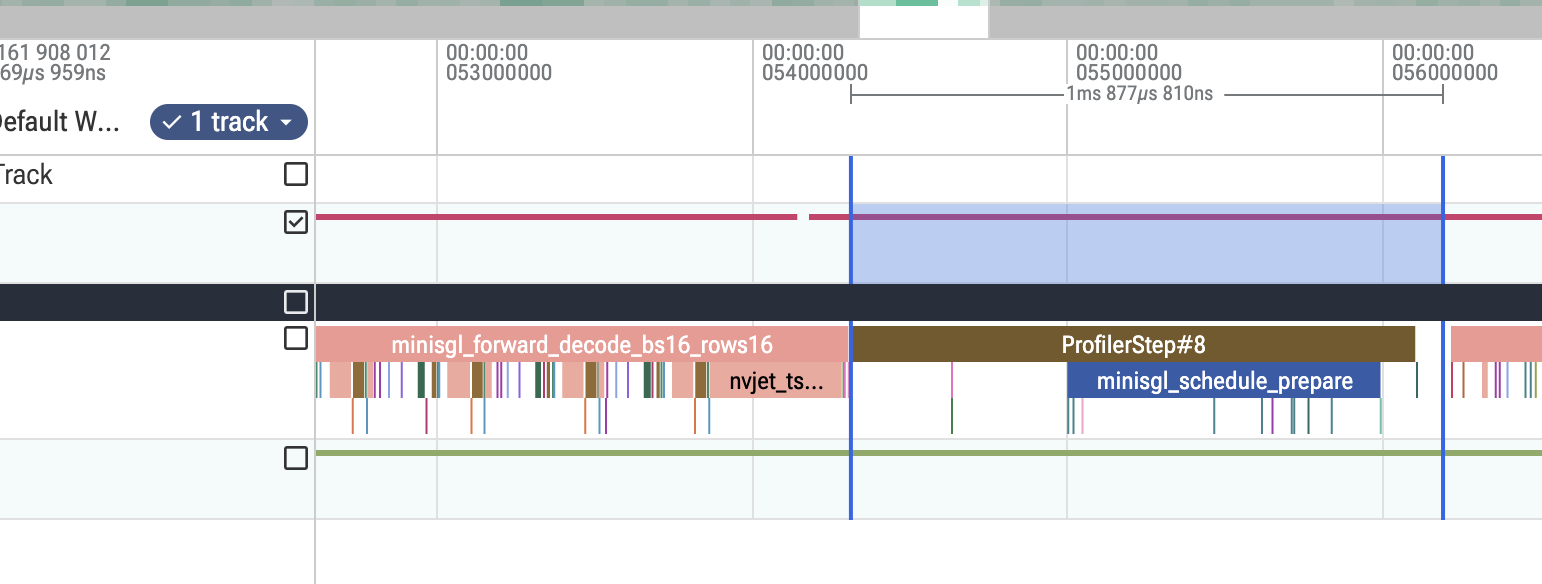
\includegraphics[width=\linewidth,height=1.68cm,keepaspectratio]
        {presentation_assets/pure-decoding-baseline.png}

      \vspace{0.18cm}
      \textbf{2. Faster n-gram lookup + batched draft-token H$\rightarrow$D}

      \vspace{0.06cm}
      \begin{center}
        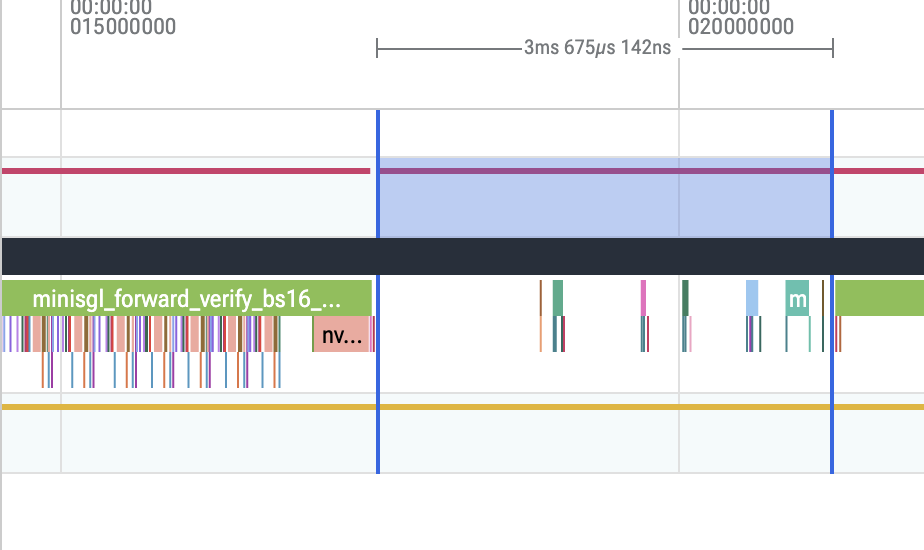
\includegraphics[width=\linewidth,height=2.05cm,keepaspectratio]
          {presentation_assets/batched-draft-htod.png}
      \end{center}
    \end{column}
    \begin{column}{0.49\textwidth}
      \textbf{1. Vanilla speculative decoding}

      \vspace{0.06cm}
      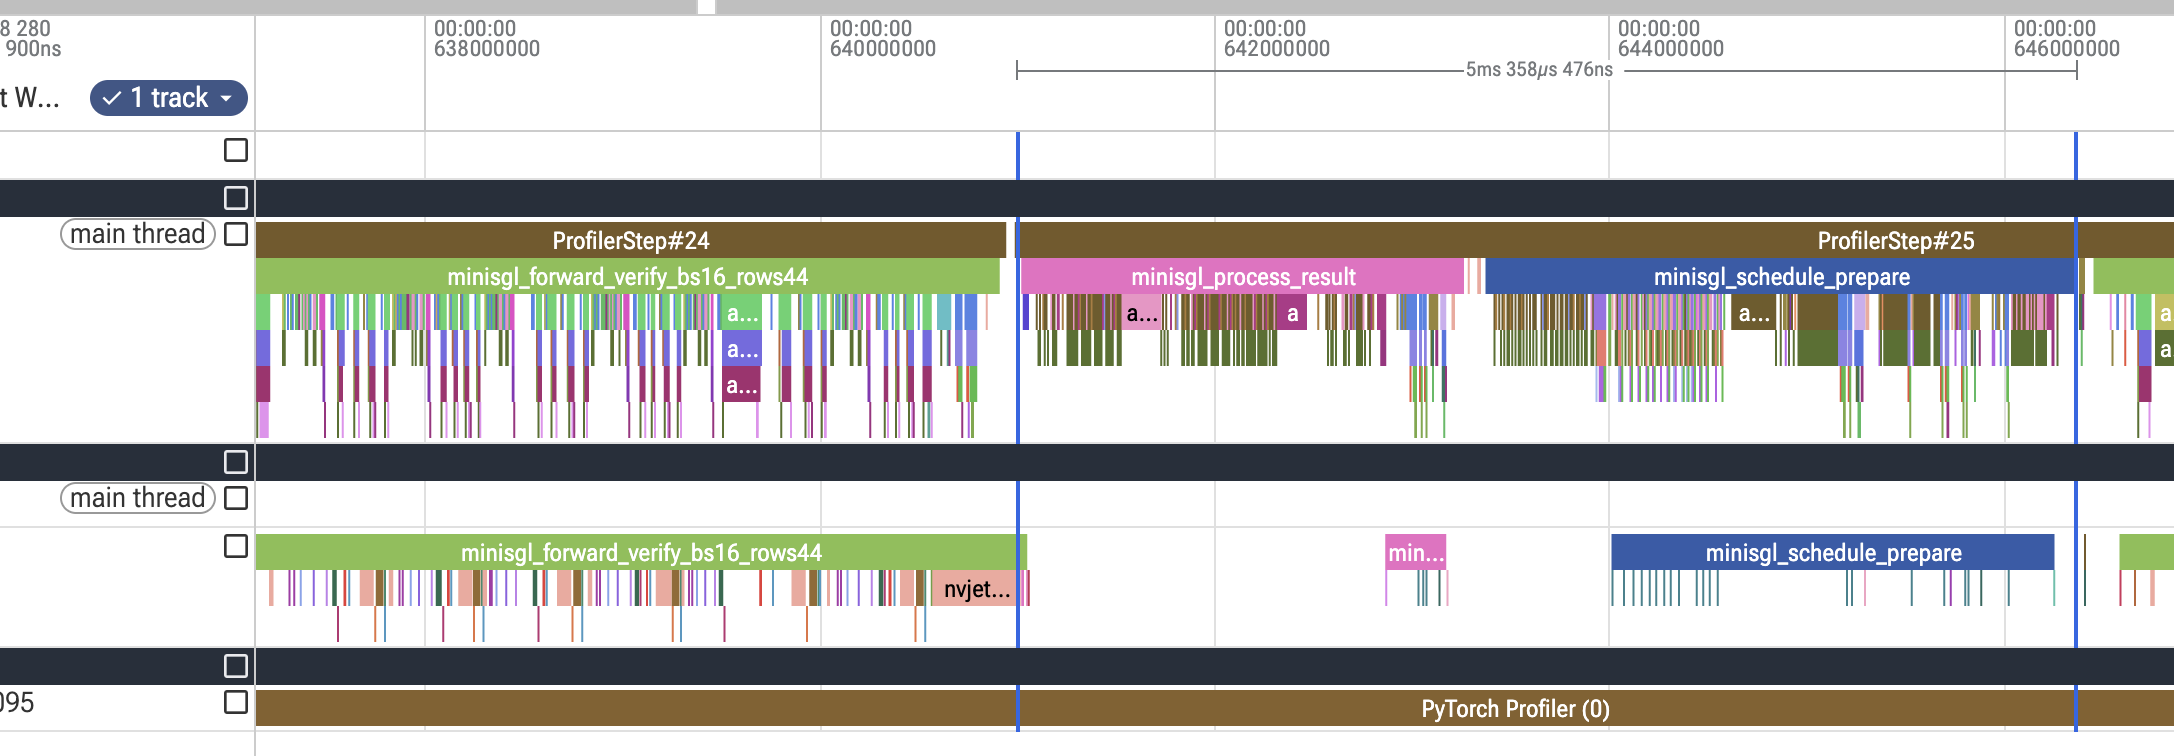
\includegraphics[width=\linewidth,height=1.68cm,keepaspectratio]
        {presentation_assets/vanilla-speculative.png}

      \vspace{0.18cm}
      \textbf{3. Batch all verification H$\rightarrow$D + misc.\ optimizations}

      \vspace{0.06cm}
      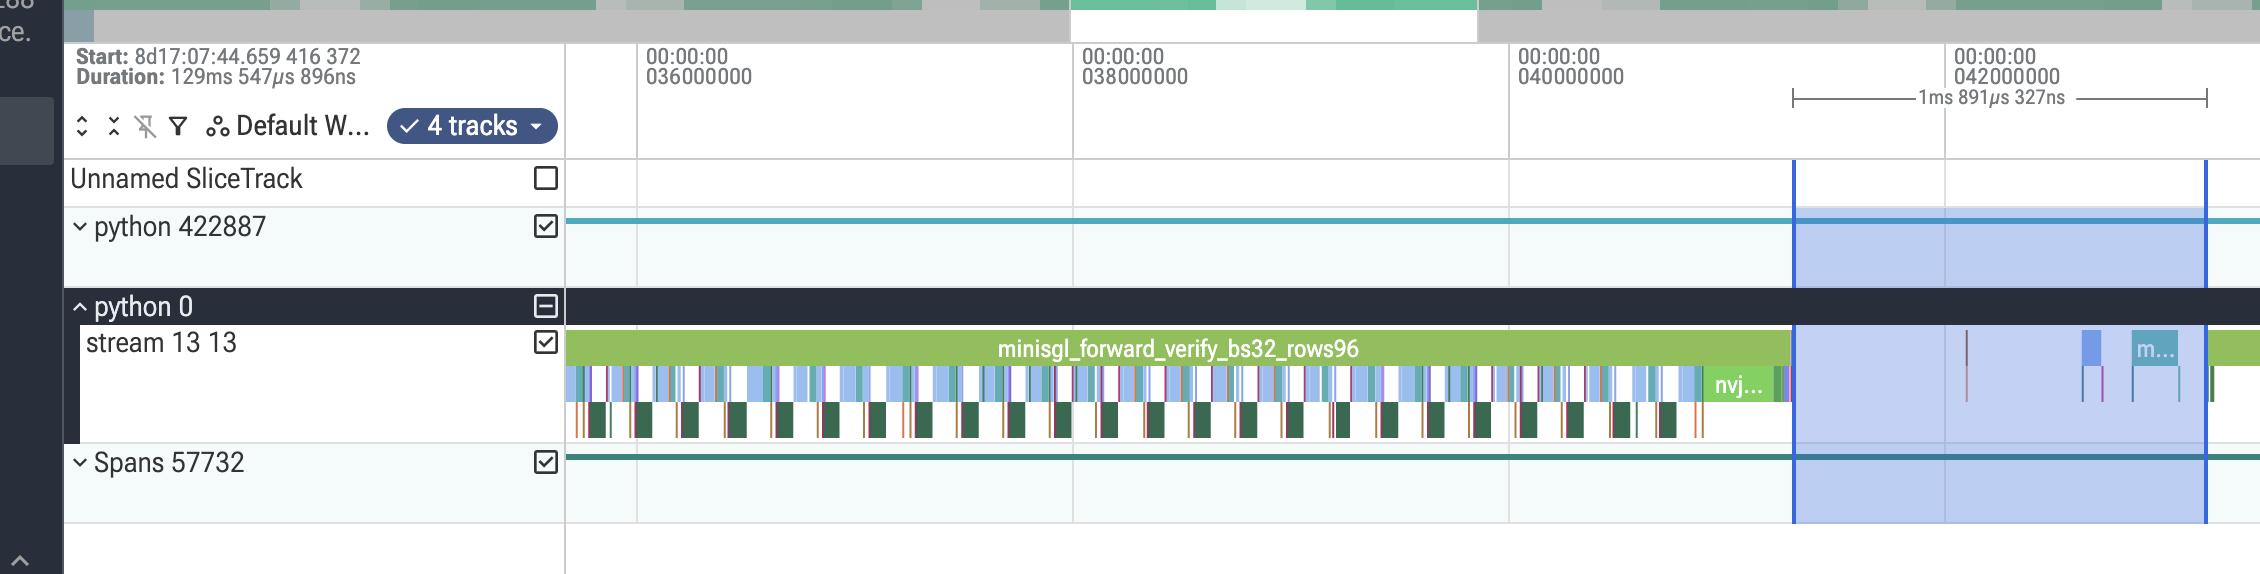
\includegraphics[width=\linewidth,height=1.68cm,keepaspectratio]
        {presentation_assets/batched-verification-htod.png}
    \end{column}
  \end{columns}
\end{frame}

\begin{frame}{CNN summarization Decode throughput vs.\ request TPOT}
  \centering
  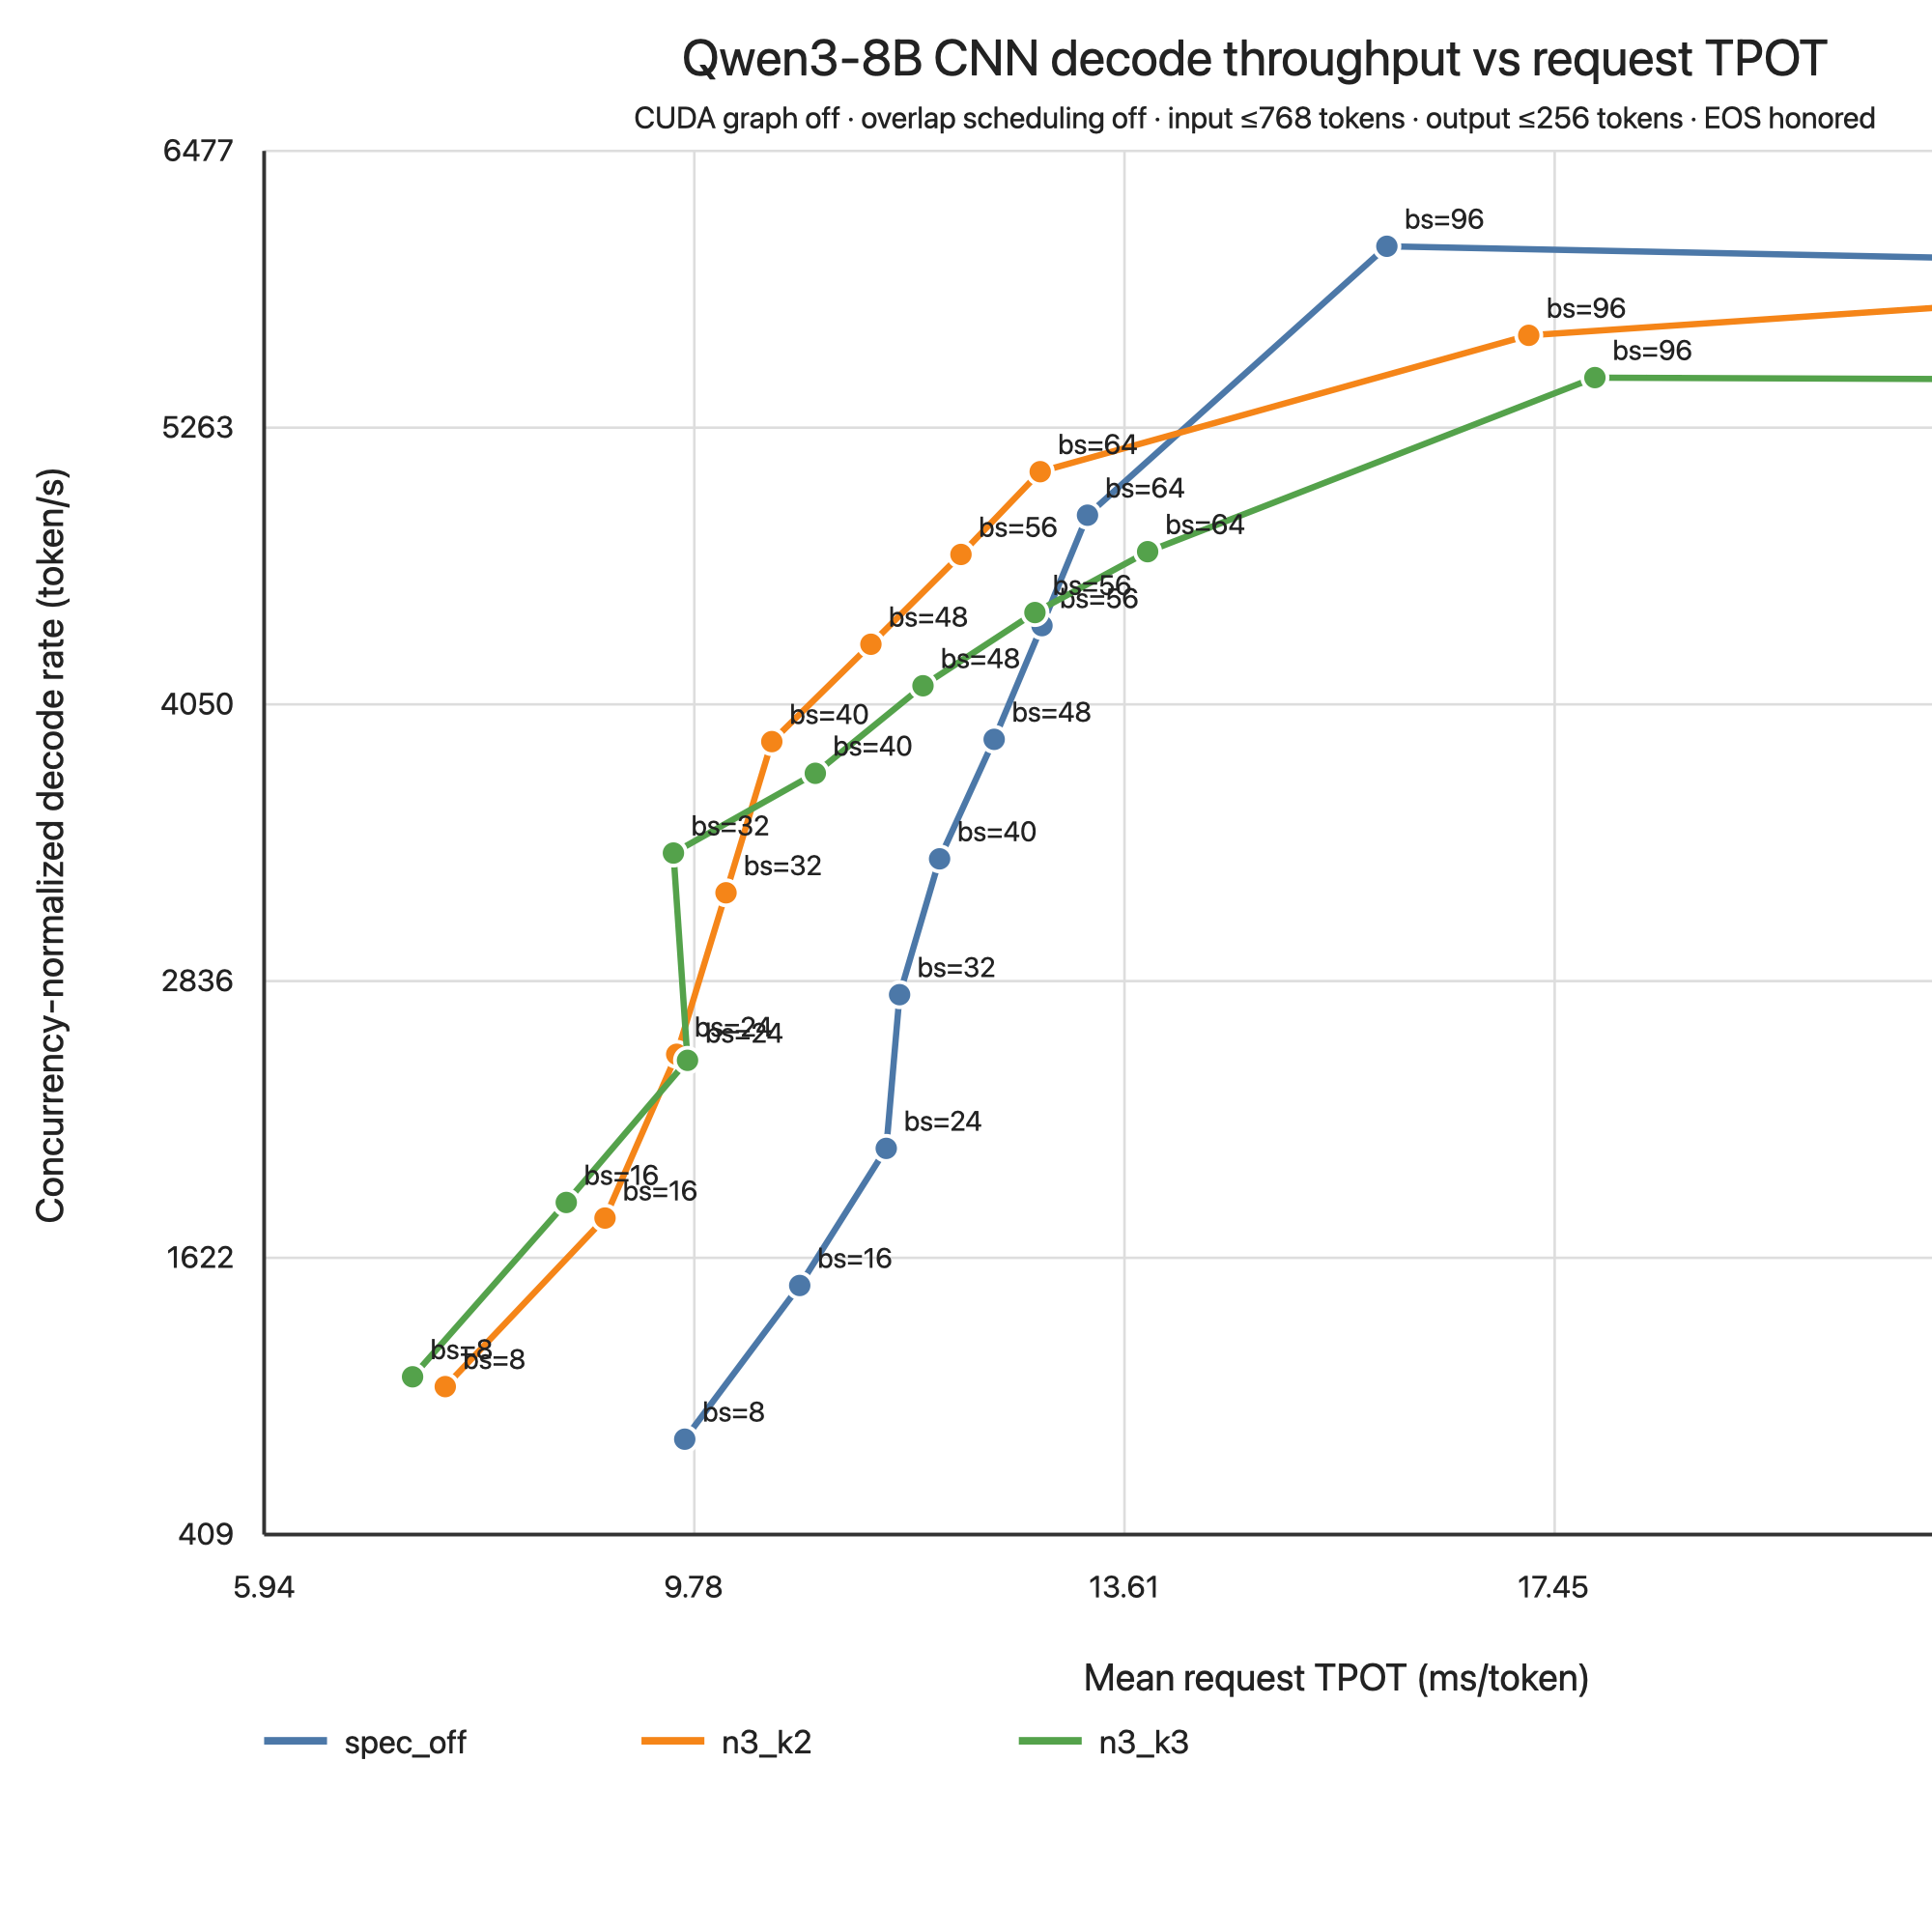
\includegraphics[width=0.88\textwidth,height=0.82\textheight,keepaspectratio]
    {presentation_assets/decode-throughput-vs-tpot.png}
\end{frame}

\begin{frame}{CNN summarization Performance summary}
  \centering
  {\small Relative to pure decoding at the same request concurrency}

  \vspace{0.03cm}
  {\scriptsize
  \renewcommand{\arraystretch}{1.05}
  \begin{tabular}{rcc|cc}
    \hline
    & \multicolumn{2}{c|}{\textbf{N=3, K=2}} &
      \multicolumn{2}{c}{\textbf{N=3, K=3}} \\
    \textbf{Concurrency} & \textbf{Throughput} & \textbf{TPOT} &
      \textbf{Throughput} & \textbf{TPOT} \\
    \hline
    8   & \textcolor{green!45!black}{+27.8\%} & \textcolor{green!45!black}{+22.0\%} & \textcolor{green!45!black}{+33.0\%} & \textcolor{green!45!black}{+25.1\%} \\
    16  & \textcolor{green!45!black}{+19.7\%} & \textcolor{green!45!black}{+16.2\%} & \textcolor{green!45!black}{+24.3\%} & \textcolor{green!45!black}{+19.4\%} \\
    24  & \textcolor{green!45!black}{+19.6\%} & \textcolor{green!45!black}{+16.3\%} & \textcolor{green!45!black}{+18.4\%} & \textcolor{green!45!black}{+15.4\%} \\
    32  & \textcolor{green!45!black}{+16.1\%} & \textcolor{green!45!black}{+13.3\%} & \textcolor{green!45!black}{+22.4\%} & \textcolor{green!45!black}{+17.4\%} \\
    40  & \textcolor{green!45!black}{+15.2\%} & \textcolor{green!45!black}{+12.5\%} & \textcolor{green!45!black}{+11.1\%} & \textcolor{green!45!black}{+9.3\%} \\
    48  & \textcolor{green!45!black}{+10.7\%} & \textcolor{green!45!black}{+8.8\%}  & \textcolor{green!45!black}{+6.0\%}  & \textcolor{green!45!black}{+5.1\%} \\
    56  & \textcolor{green!45!black}{+7.1\%}  & \textcolor{green!45!black}{+5.6\%}  & \textcolor{green!45!black}{+1.3\%}  & \textcolor{green!45!black}{+0.5\%} \\
    64  & \textcolor{green!45!black}{+3.9\%}  & \textcolor{green!45!black}{+3.2\%}  & \textcolor{red!70!black}{-3.3\%}    & \textcolor{red!70!black}{-4.0\%} \\
    96  & \textcolor{red!70!black}{-6.4\%}    & \textcolor{red!70!black}{-7.9\%}    & \textcolor{red!70!black}{-9.5\%}    & \textcolor{red!70!black}{-11.6\%} \\
    128 & \textcolor{red!70!black}{-2.7\%}    & \textcolor{red!70!black}{-3.1\%}    & \textcolor{red!70!black}{-8.8\%}    & \textcolor{red!70!black}{-10.0\%} \\
    \hline
  \end{tabular}}

  \vspace{0.08cm}
  \textbf{Acceptance statistics}

  \vspace{0.02cm}
  {\footnotesize
  \renewcommand{\arraystretch}{1.0}
  \begin{tabular}{lcccc}
    \hline
    \textbf{Draft length} & \textbf{Mean accepted} & \textbf{p0} & \textbf{p1} & \textbf{p2} \\
    \hline
    $K=2$ & 0.52 & 32.78\% & 57.27\% & --- \\
    $K=3$ & 0.59 & 31.22\% & 57.27\% & 57.93\% \\
    \hline
  \end{tabular}}

  \vspace{0.03cm}
  {\scriptsize Mean accepted = draft tokens per verification step. TPOT = mean
  request time per output token. Later draft-position acceptance is conditional
  on every earlier position being accepted.}
\end{frame}

\begin{frame}{Numerical test results}
  \begin{columns}[T,onlytextwidth]
    \begin{column}{0.42\textwidth}
      \vspace{0.35cm}
      \textbf{Test configuration}

      \vspace{0.16cm}
      \begin{itemize}
        \setlength{\itemsep}{0.25cm}
        \item FlashInfer backend
        \item 2,000 CNN/DailyMail cases
        \item Batch size 8; greedy decoding
        \item $N=3$, $K=4$; 32 generated tokens
        \item EOS ignored
      \end{itemize}
    \end{column}
    \begin{column}{0.53\textwidth}
      \vspace{0.35cm}
      \textbf{Observed against pure decoding}

      \vspace{0.17cm}
      {\Large\textcolor{red!70!black}{385 / 2,000 requests}}

      \vspace{0.03cm}
      had a token mismatch (\textbf{19.25\%}); the strict exact-token test failed.

      \vspace{0.35cm}
      \begin{tabular}{lr}
        Compared token log-probabilities & 59,066 \\
        Mean $|\Delta \log p|$ & 0.00859 \\
        P99 $|\Delta \log p|$ & 0.07795 \\
        Maximum $|\Delta \log p|$ & 0.19228 \\
      \end{tabular}

      \vspace{0.12cm}
      {\tiny Separate EOS-honored CNN run, batch size 128 (128 traces):
      exact completion matches were \textbf{84 / 128} for $N=3,K=2$ and
      \textbf{90 / 128} for $N=3,K=3$.}
    \end{column}
  \end{columns}

  \vspace{0.18cm}
  \begin{block}{Batch-size sensitivity}
    Main SGLang reproduces the instability on \textbf{50 / 50 adversarial
    prompts} at batch size 1; batch size 8 is not stable. The effect is
    batch-size sensitive.
  \end{block}
\end{frame}

\begin{frame}{CNN exact mismatch example 1 (BS=128)}
  \scriptsize
  \textcolor{black!65}{Article ID: 7fdbcd9bd3ea48687457817b6440183837d97c85. First differing character: 37.}

  \vspace{0.16cm}
  \begin{columns}[T,onlytextwidth]
    \begin{column}{0.48\textwidth}
      \textbf{Spec-off}
      \begin{itemize}\setlength{\itemsep}{0.22cm}
        \item Daryl Janmaat compared Newcastle's upcoming Premier League match against Swansea to a World Cup semi-final due to its significance.
        \item Newcastle has lost their last six league games, leaving them seven points above the relegation zone with five games remaining.
        \item Janmaat, who played in the 2014 World Cup semi-final, emphasized the importance of winning to ensure safety from relegation.
      \end{itemize}
    \end{column}
    \begin{column}{0.48\textwidth}
      \textbf{$N=3$, $K=2$ speculative}
      \begin{itemize}\setlength{\itemsep}{0.22cm}
        \item Daryl Janmaat compared Newcastle's Premier League match against Swansea to a World Cup semi-final due to its significance.
        \item Newcastle has lost their last six league games and is seven points above the relegation zone with five games remaining.
        \item Janmaat, who played in the 2014 World Cup semi-final, emphasized the importance of winning to ensure safety from relegation.
      \end{itemize}
    \end{column}
  \end{columns}
\end{frame}

\begin{frame}{CNN exact mismatch: second example (BS=128)}
  \scriptsize
  \textcolor{black!65}{Article ID: 0ecc8cb598f4bdee432dd9d5de63bd64d74eb794. First differing character: 45.}

  \vspace{0.16cm}
  \begin{columns}[T,onlytextwidth]
    \begin{column}{0.48\textwidth}
      \textbf{Spec-off}
      \begin{itemize}\setlength{\itemsep}{0.22cm}
        \item James Lockwood received a two-year ban for doping after testing positive for Growth Hormone Releasing Peptide-2 (pralmorelin) in an out-of-competition test.
        \item The ban, the first of its kind in the UK, starts on 3 March 2015 and ends on 2 March 2017.
        \item Lockwood, a 29-year-old Featherstone player, joined the team in 2012 and was part of the squad that lost the Championship Grand Final in October 2014.
      \end{itemize}
    \end{column}
    \begin{column}{0.48\textwidth}
      \textbf{$N=3$, $K=2$ speculative}
      \begin{itemize}\setlength{\itemsep}{0.22cm}
        \item James Lockwood received a two-year ban for failing a doping test, marking the first such case in the UK under the Rugby Football League's anti-doping regulations.
        \item The positive test result was for Growth Hormone Releasing Peptide-2 (pralmorelin) and its metabolite, identified in an out-of-competition sample from November 2014.
        \item Lockwood, a 29-year-old Featherstone prop, is suspended from all competition from 3 March 2015 to 2 March 2017.
      \end{itemize}
    \end{column}
  \end{columns}
\end{frame}

\begin{frame}{MATH-500 decode throughput vs.\ request TPOT}
  \centering
  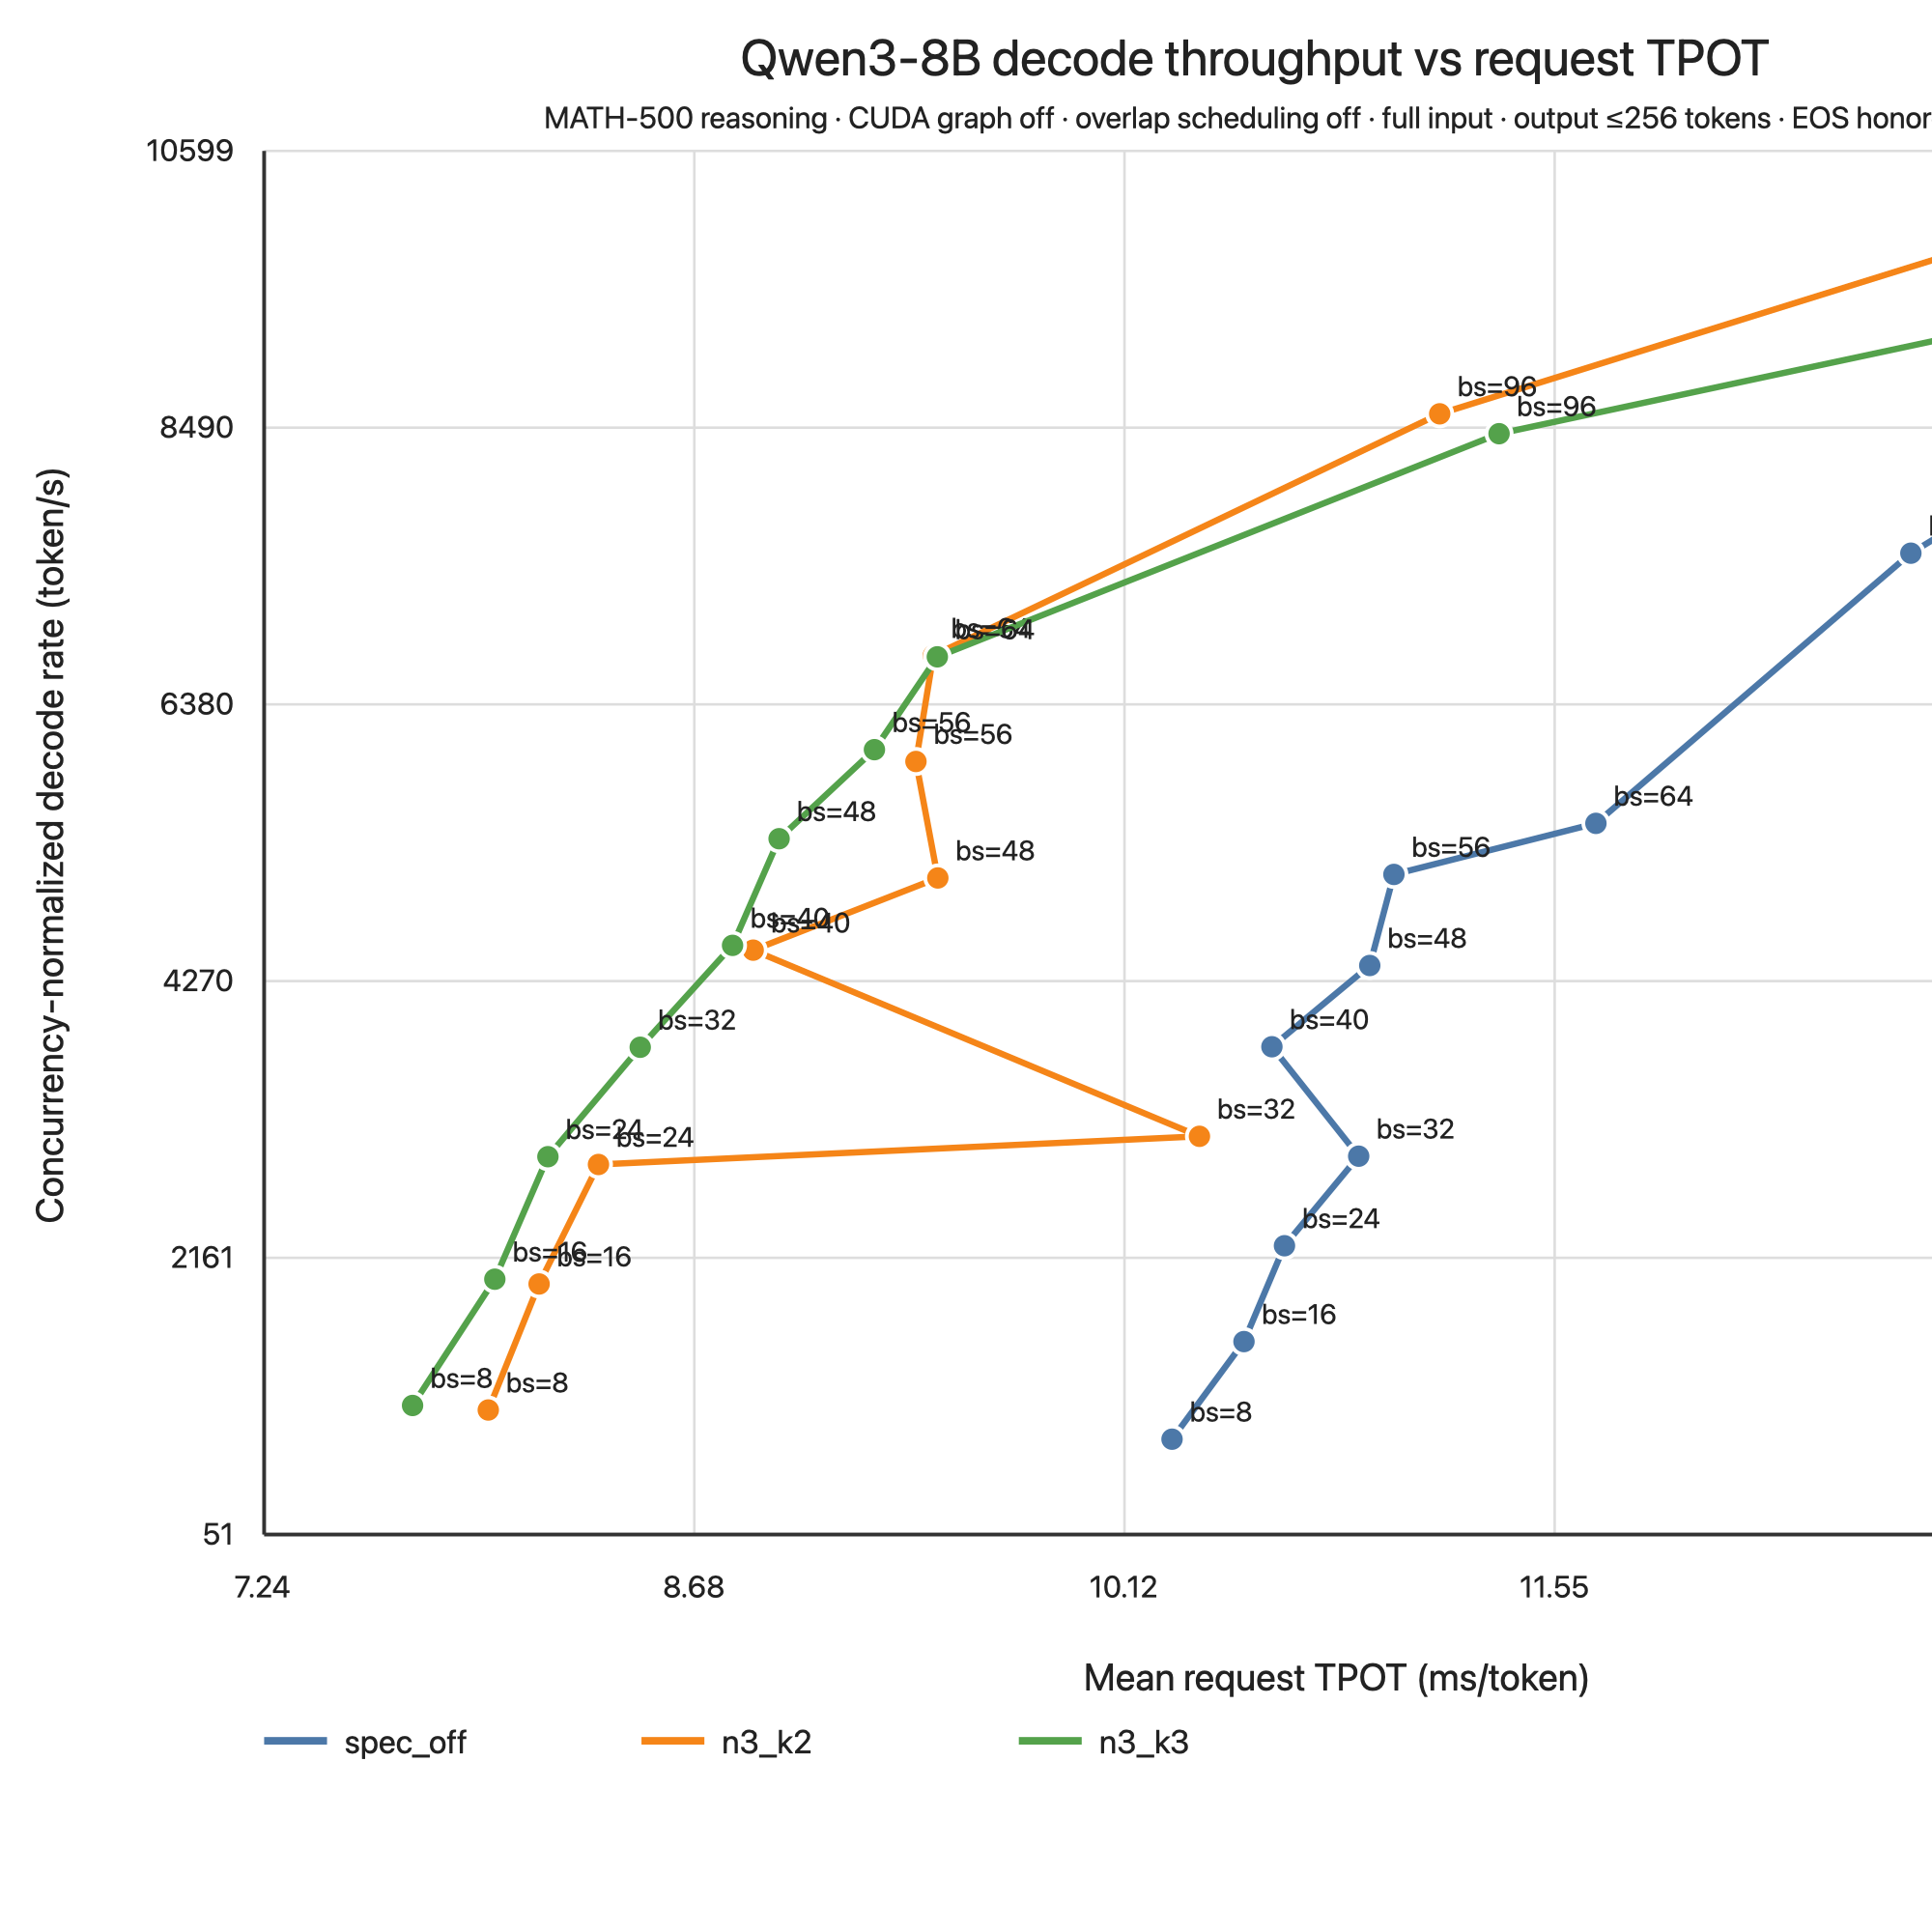
\includegraphics[width=0.88\textwidth,height=0.82\textheight,keepaspectratio]
    {presentation_assets/math500-decode-throughput-vs-tpot.png}
\end{frame}

\begin{frame}{MATH-500 reasoning performance summary}
  \centering
  {\small 500 fixed problems per point; reasoning enabled; full input; EOS honored;
  CUDA graph and overlap scheduling disabled.}

  \vspace{0.08cm}
  {\scriptsize Relative to pure decoding at the same request concurrency
  \renewcommand{\arraystretch}{1.03}
  \begin{tabular}{rcc|cc}
    \hline
    & \multicolumn{2}{c|}{\textbf{N=3, K=2}} &
      \multicolumn{2}{c}{\textbf{N=3, K=3}} \\
    \textbf{Concurrency} & \textbf{Throughput} & \textbf{TPOT} &
      \textbf{Throughput} & \textbf{TPOT} \\
    \hline
    8   & \textcolor{green!45!black}{+28.6\%} & \textcolor{green!45!black}{+22.2\%} & \textcolor{green!45!black}{+32.8\%} & \textcolor{green!45!black}{+24.7\%} \\
    16  & \textcolor{green!45!black}{+28.9\%} & \textcolor{green!45!black}{+22.4\%} & \textcolor{green!45!black}{+31.3\%} & \textcolor{green!45!black}{+23.8\%} \\
    24  & \textcolor{green!45!black}{+27.4\%} & \textcolor{green!45!black}{+21.5\%} & \textcolor{green!45!black}{+30.1\%} & \textcolor{green!45!black}{+23.1\%} \\
    32  & \textcolor{green!45!black}{+5.1\%}  & \textcolor{green!45!black}{+4.9\%}  & \textcolor{green!45!black}{+28.3\%} & \textcolor{green!45!black}{+22.0\%} \\
    40  & \textcolor{green!45!black}{+19.5\%} & \textcolor{green!45!black}{+16.3\%} & \textcolor{green!45!black}{+20.5\%} & \textcolor{green!45!black}{+17.0\%} \\
    48  & \textcolor{green!45!black}{+15.2\%} & \textcolor{green!45!black}{+13.2\%} & \textcolor{green!45!black}{+22.0\%} & \textcolor{green!45!black}{+18.1\%} \\
    56  & \textcolor{green!45!black}{+17.0\%} & \textcolor{green!45!black}{+14.5\%} & \textcolor{green!45!black}{+18.7\%} & \textcolor{green!45!black}{+15.8\%} \\
    64  & \textcolor{green!45!black}{+23.4\%} & \textcolor{green!45!black}{+18.9\%} & \textcolor{green!45!black}{+23.2\%} & \textcolor{green!45!black}{+18.8\%} \\
    96  & \textcolor{green!45!black}{+14.1\%} & \textcolor{green!45!black}{+12.4\%} & \textcolor{green!45!black}{+12.1\%} & \textcolor{green!45!black}{+10.8\%} \\
    128 & \textcolor{green!45!black}{+7.5\%}  & \textcolor{green!45!black}{+7.0\%}  & \textcolor{green!45!black}{+3.2\%}  & \textcolor{green!45!black}{+3.1\%} \\
    \hline
  \end{tabular}}

  \vspace{0.14cm}
  \textbf{Acceptance statistics}

  \vspace{0.04cm}
  {\footnotesize
  \begin{tabular}{lcccc}
    \hline
    \textbf{Draft length} & \textbf{Mean accepted} & \textbf{p0} & \textbf{p1} & \textbf{p2} \\
    \hline
    $K=2$ & 0.43 & 28.64\% & 52.05\% & --- \\
    $K=3$ & 0.49 & 27.23\% & 50.92\% & 59.17\% \\
    \hline
  \end{tabular}}
\end{frame}

\begin{frame}{CUDA graphs + overlapped scheduling}
  \centering
  \textcolor{black!65}{CUDA graph enabled \quad$\cdot$\quad overlap scheduling enabled}

  \vspace{0.2cm}
  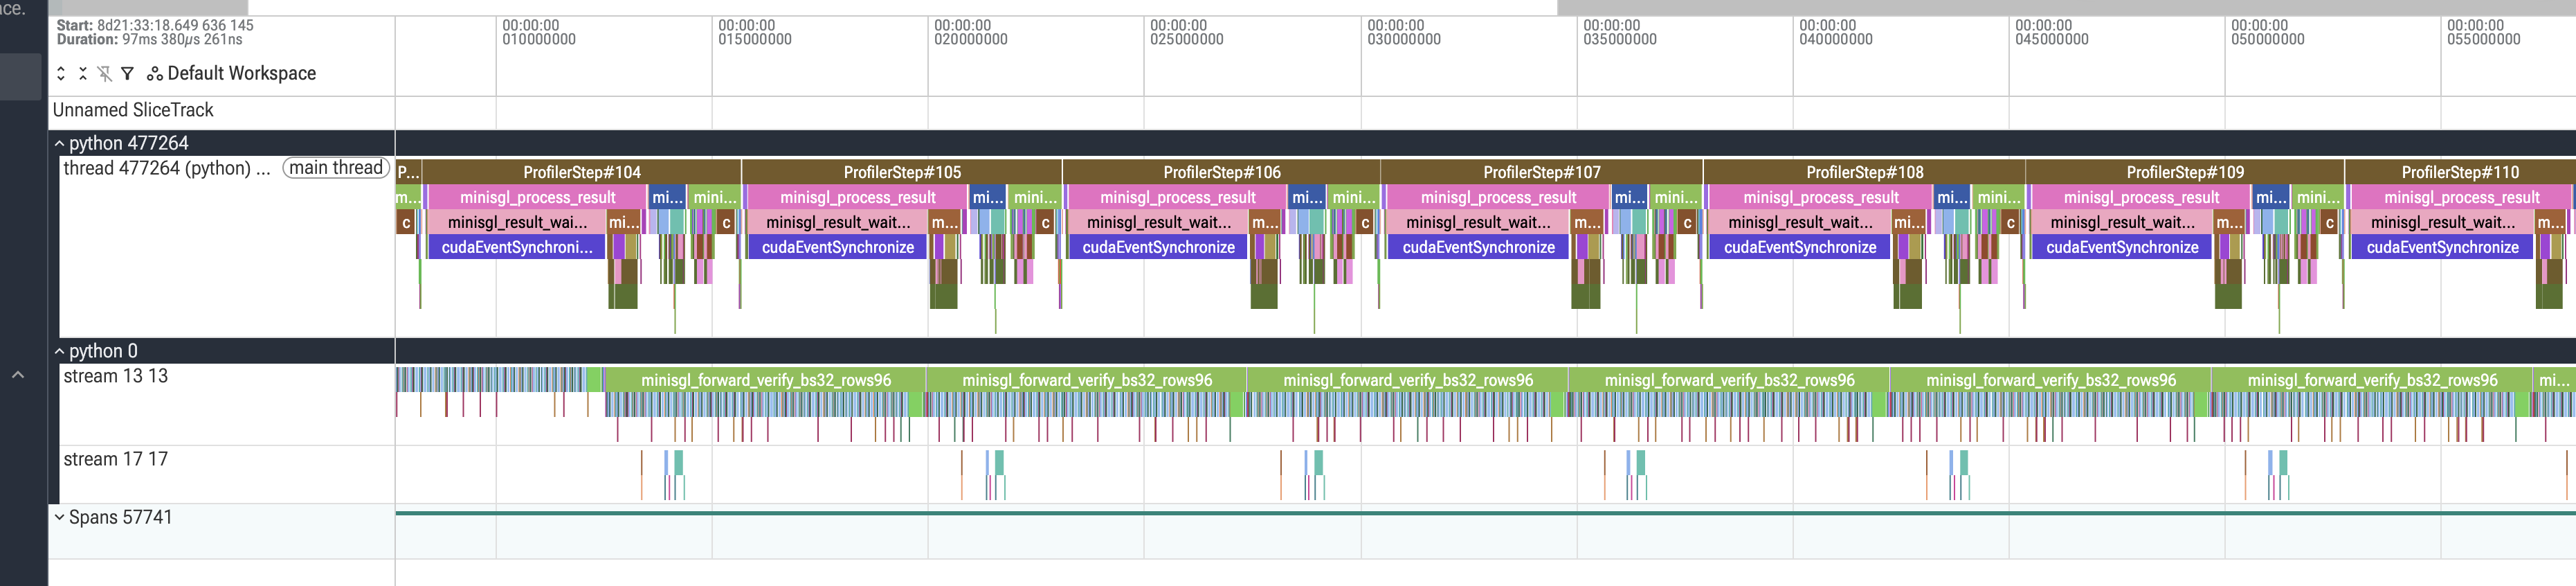
\includegraphics[width=0.96\textwidth,height=0.72\textheight,keepaspectratio]
    {presentation_assets/cuda-graph-overlap-trace.png}
\end{frame}

\begin{frame}{N-gram rejection sampling: deterministic proposal}
  \centering
  \begin{tikzpicture}[
      >=Latex,
      flow/.style={->, very thick, draw=black!60},
      box/.style={draw=blue!70!black, very thick, rounded corners=4pt,
        fill=blue!9, minimum width=2.55cm, minimum height=1.2cm, align=center},
      acceptbox/.style={draw=green!45!black, very thick, rounded corners=4pt,
        fill=green!10, minimum width=2.7cm, minimum height=1.2cm, align=center},
      rejectbox/.style={draw=red!70!black, very thick, rounded corners=4pt,
        fill=red!9, minimum width=3.15cm, minimum height=1.2cm, align=center},
      heading/.style={font=\large\bfseries, text=blue!75!black},
      note/.style={font=\small, align=center, text=black!65}
    ]
    \node[heading] at (-4.2,2.0) {N-gram lookup};
    \node[box] (draft) at (-4.2,0.95)
      {\textbf{Draft token } $d$\\[2pt]\large $q(d)=1$};
    \node[note] at (-4.2,-0.1)
      {$q(v)=0$ for every $v \ne d$};

    \draw[flow] (draft.east) -- (0.0,0.95);
    \node[heading] at (0.95,2.0) {Target sampling};
    \node[box, minimum width=2.35cm] (target) at (0.95,0.95)
      {\textbf{Draw } $z \sim p_\theta$\\[2pt]
       \small from the target distribution};

    \node[acceptbox, minimum width=2.3cm, minimum height=1.0cm] (accept) at (4.65,1.55)
      {\textbf{If $z=d$}\\[2pt] accept the draft token};
    \node[rejectbox, minimum width=2.65cm, minimum height=1.0cm] (reject) at (4.65,-0.3)
      {\textbf{If $z\ne d$}\\[2pt] reject $d$ and emit $z$};
    \draw[flow] (target.east) -- (accept.west);
    \draw[flow] (target.east) -- (reject.west);

    \node[draw=black!55, rounded corners=4pt, fill=gray!5,
      minimum width=10.8cm, minimum height=1.0cm, align=center] at (0,-2.0)
      {\textbf{Why $q=1$ matters:}\quad
       $\Pr[\mathrm{accept}]=p_\theta(d\mid h)$,\qquad
       $z\mid z\ne d \sim \dfrac{p_\theta(z\mid h)}{1-p_\theta(d\mid h)}
       \quad (z\ne d)$};
    \node[note] at (0,-2.8)
      {Apply the same rule left-to-right over the draft; stop at the first rejection.};
  \end{tikzpicture}
\end{frame}

\end{document}
